
%Copyright (C) 2016 by Krishneel@JSK Lab, The University of Tokyo

\documentclass{standalone}
\begin{document}

\subsection{Platforms}
For task 3, we developed two types of UAVs. We first used customized DJI M100 as our standard platform\ref{task3platform-m100} which had been introduced in task 1. We equipped Nvidia Jetson TX1 and TK1 based embedded computer to do both control and vision algorithms. The magnets gripper is redesigned to be stronger to pick the objects and also for the drone to fly more stable. For the second type, we improved the transformable aerial robot called {\bf Hydrus} \ref{task3platform-hydrus} as described in the first report. The propeller of  {\bf Hydrus} is 14[inch] which is much bigger than the prototpye, leading to the improvement of the flight performance. Temporarily we did the real world test through remote operation with the standard platform, we are also trying to set up the network configurations which is given by the MBZIRC committee recently. Also we accelerate our vision algorithm in gazebo simulation as we showed in the first report. For now we are trying to develop a semi-autonomous approach for task 3 considering the difficulties we meet in manually operation.
 \begin{figure}%[hb]
    \begin{center}
    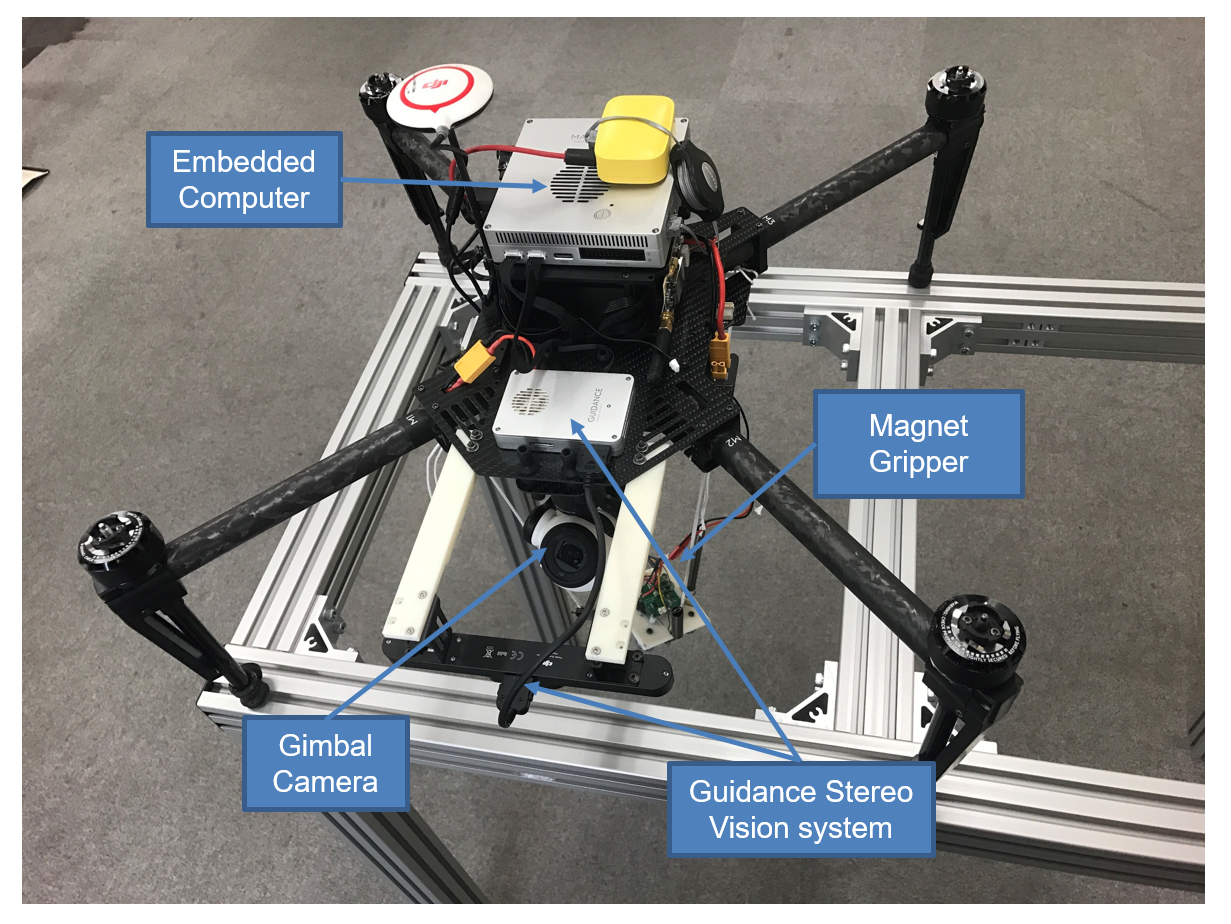
\includegraphics[keepaspectratio=true, width=1\linewidth, height=0.3\textheight]
    {sections//task3//images//task3platform.png}
      \end{center}
    \caption{Task 3 Platform: DJI M100}
    \label{task3platform-m100}
    \end{figure}
 \begin{figure}%[hb]
    \begin{center}
      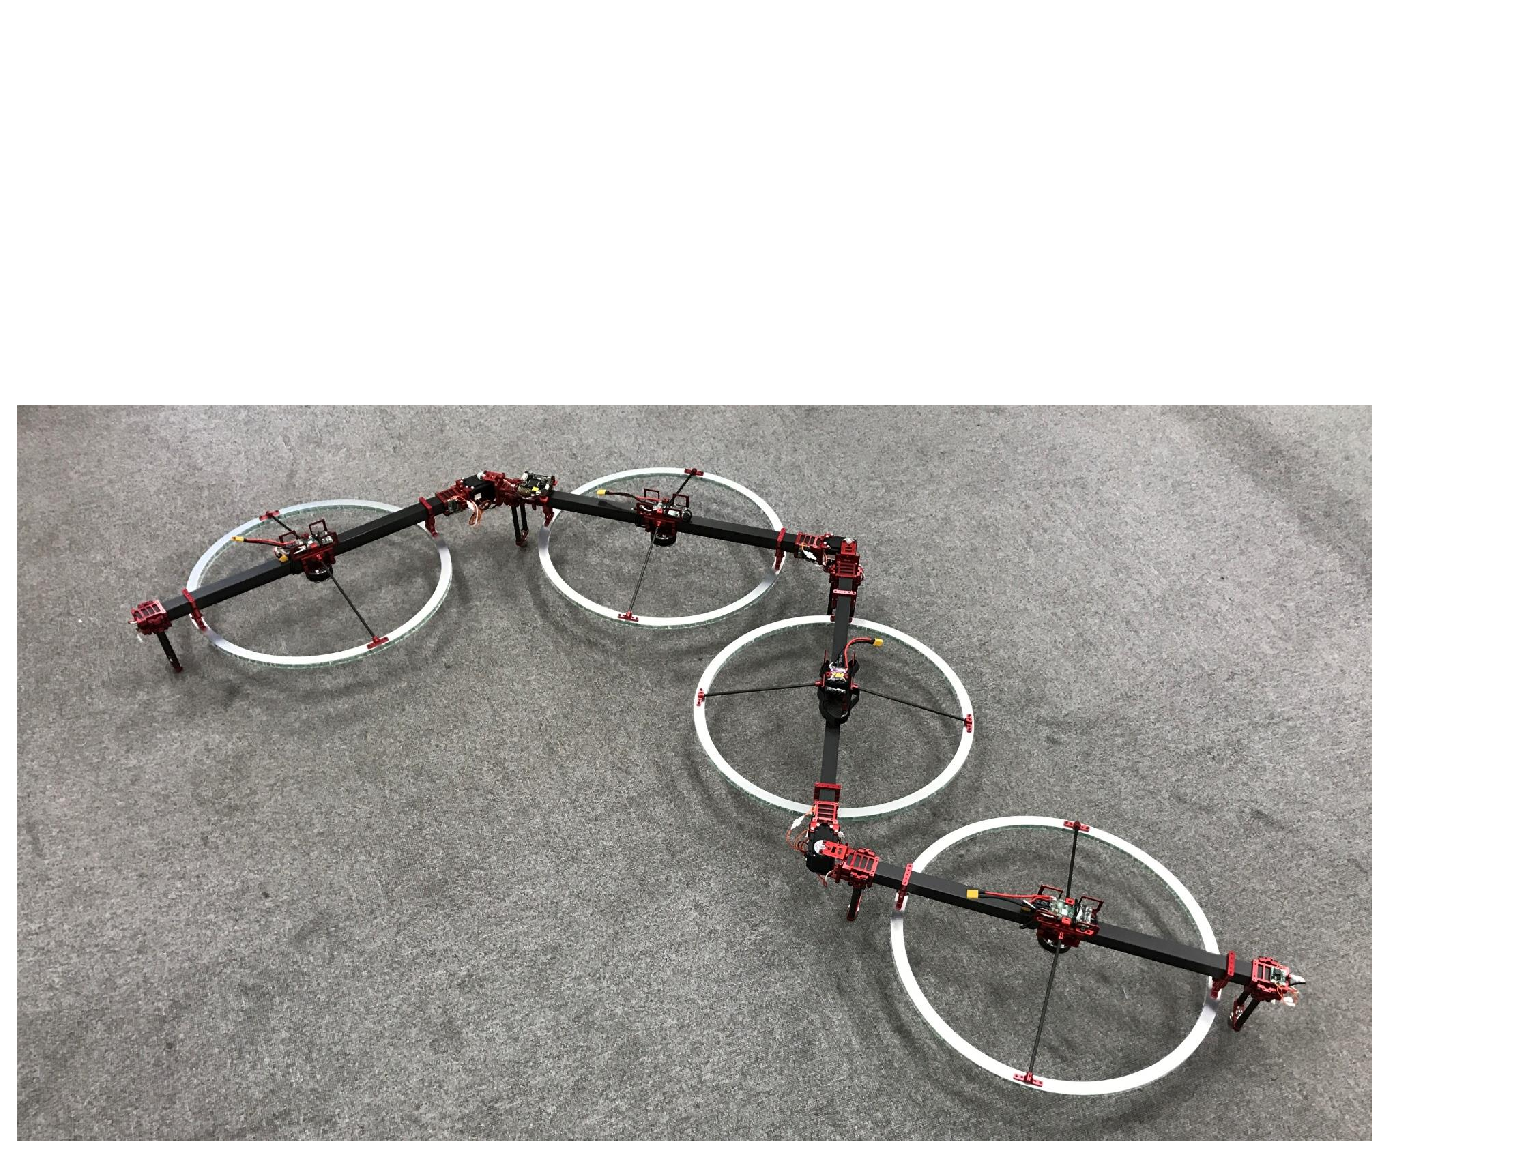
\includegraphics[clip, bb= 0 0 650 350, width=\columnwidth]{sections/task3/images/task3platform-hydrus.eps}
      \end{center}
    \caption{Task 3 Platform: Hydrus}
    \label{task3platform-hydrus}
    \end{figure}
    
    
\subsection{Electromagnet Gripper for Quadcopter}
The reason we choose electromagnet is that it is easy to control if we design the circuits ourselves. The ordinary seems stronger but it may requires executor unit to push the object down when the drone will to release the object, which will make the attachment more complex and additional motor is needed. We also considered to use a air vacuum like our team in Amazon Picking Challenge, but the size of vacuum is too big for the drone in our case. 
 \begin{figure}[hb]
    \begin{center}
    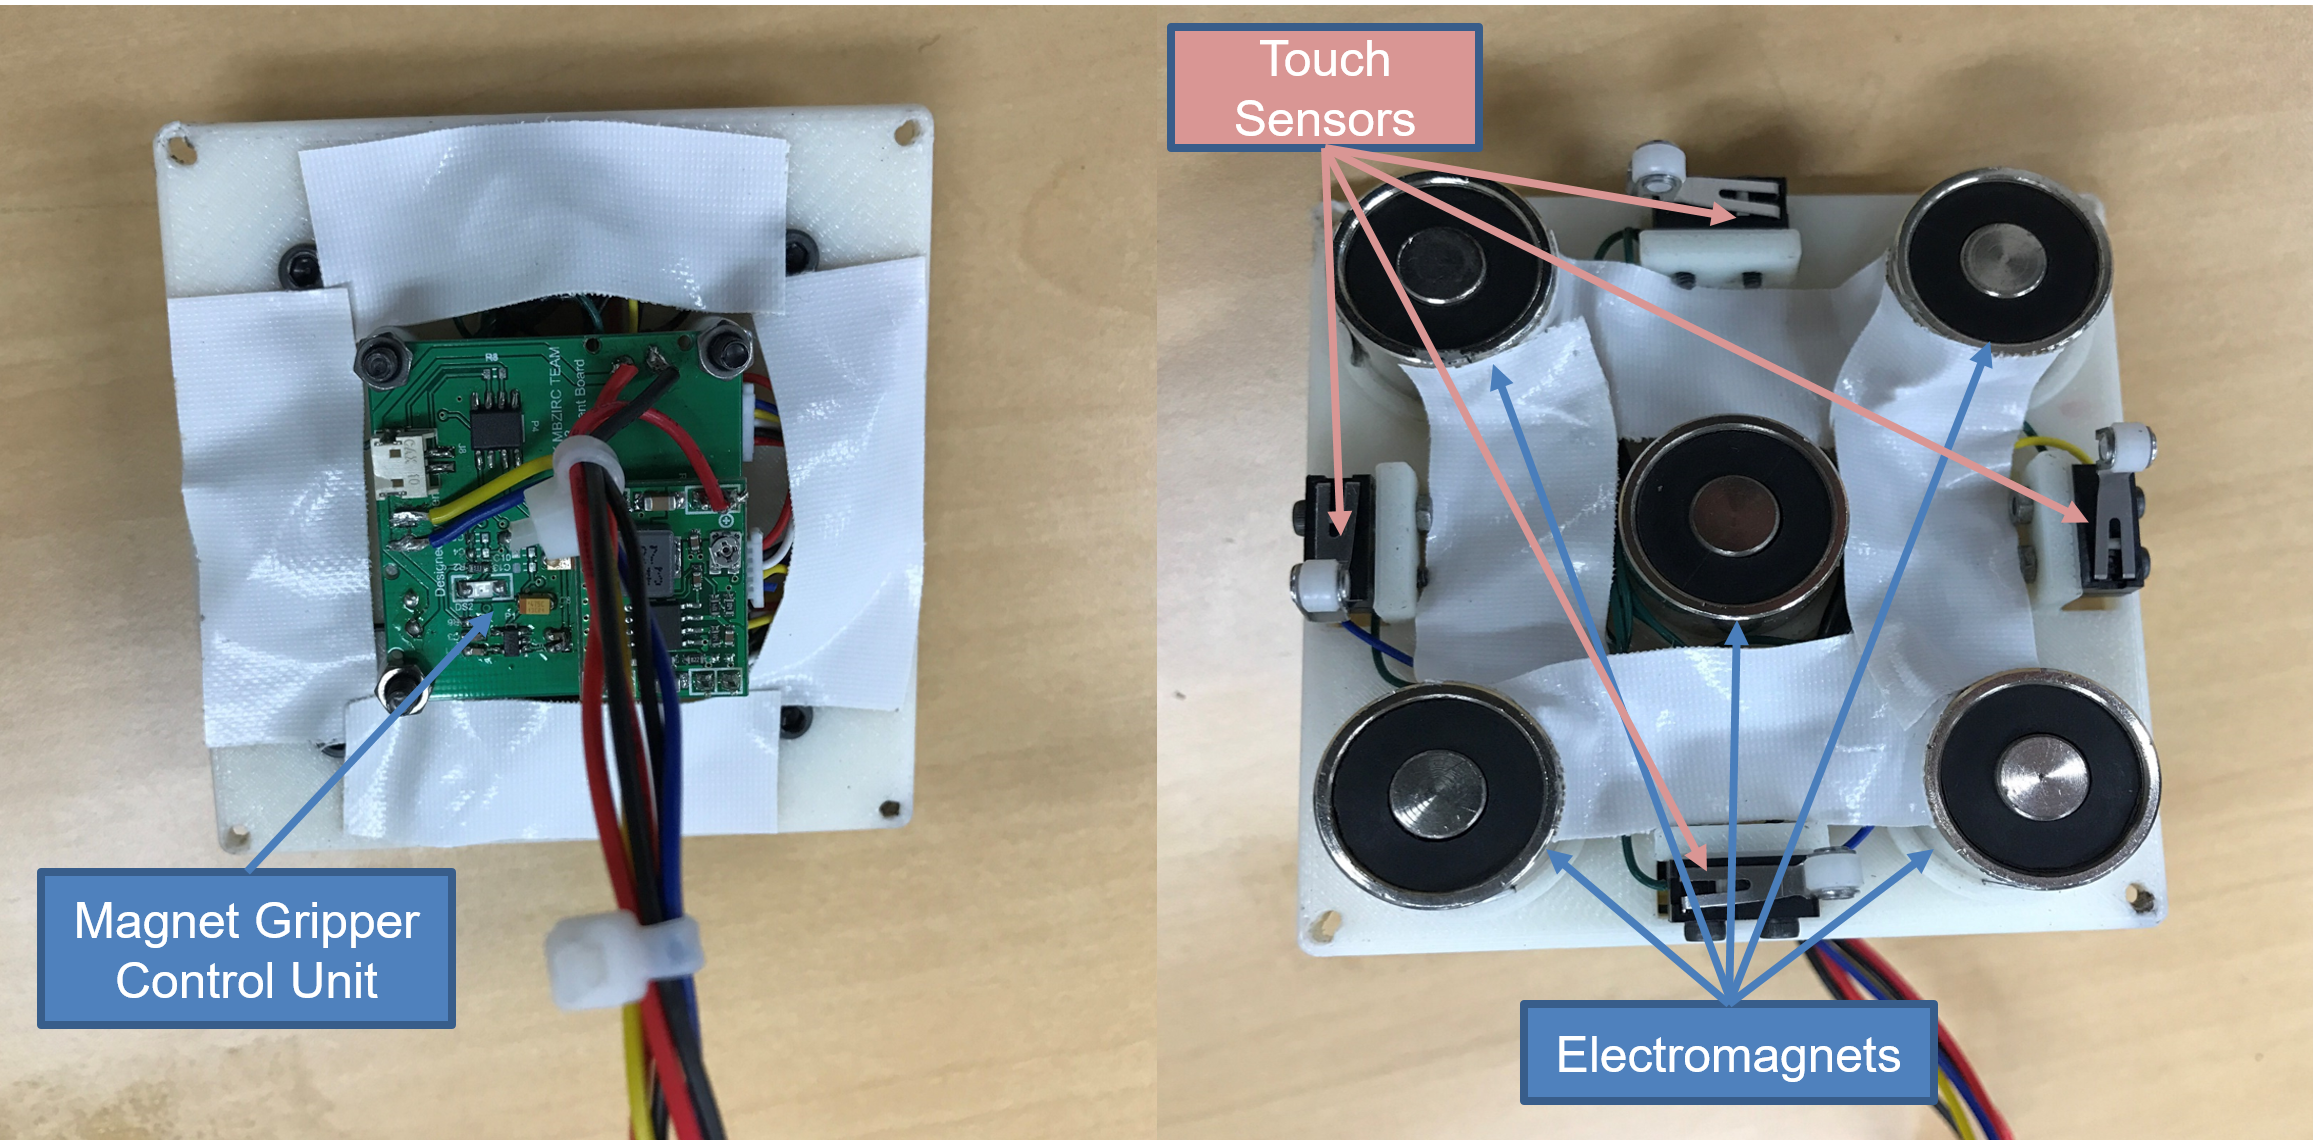
\includegraphics[keepaspectratio=true, width=1\linewidth, height=0.3\textheight]
    {sections//task3//images//task3gripper.png}
      \end{center}
    \caption{Task 3 Gripper($8cm \times 8cm, 240g$)}
    \label{task3platform}
    \end{figure}

We equipped 5 small electromagnets for a gripper of size $8cm \times 8cm$. Each electromagnet is capable of more than $20 N$ holding force if the objects are thick enough. However, according to our experiment, since each object is less than $500 g$, the thickness will be less than $1.6 mm$ if the object is a square of $20cm \times 20cm$ and made of pure iron(consider the density of iron to be $7.86 g/cm$). In addition, if the surface of the object is too large, the propeller effect will happen and therefore request the electromagnets to be more powerful. Temporary our gripper with $5$ electromagnets can pick the object of almost $1kg$ of the thickness of the iron is more than $0.3mm$. 
 \begin{figure*}%[hb]
    \begin{center}
    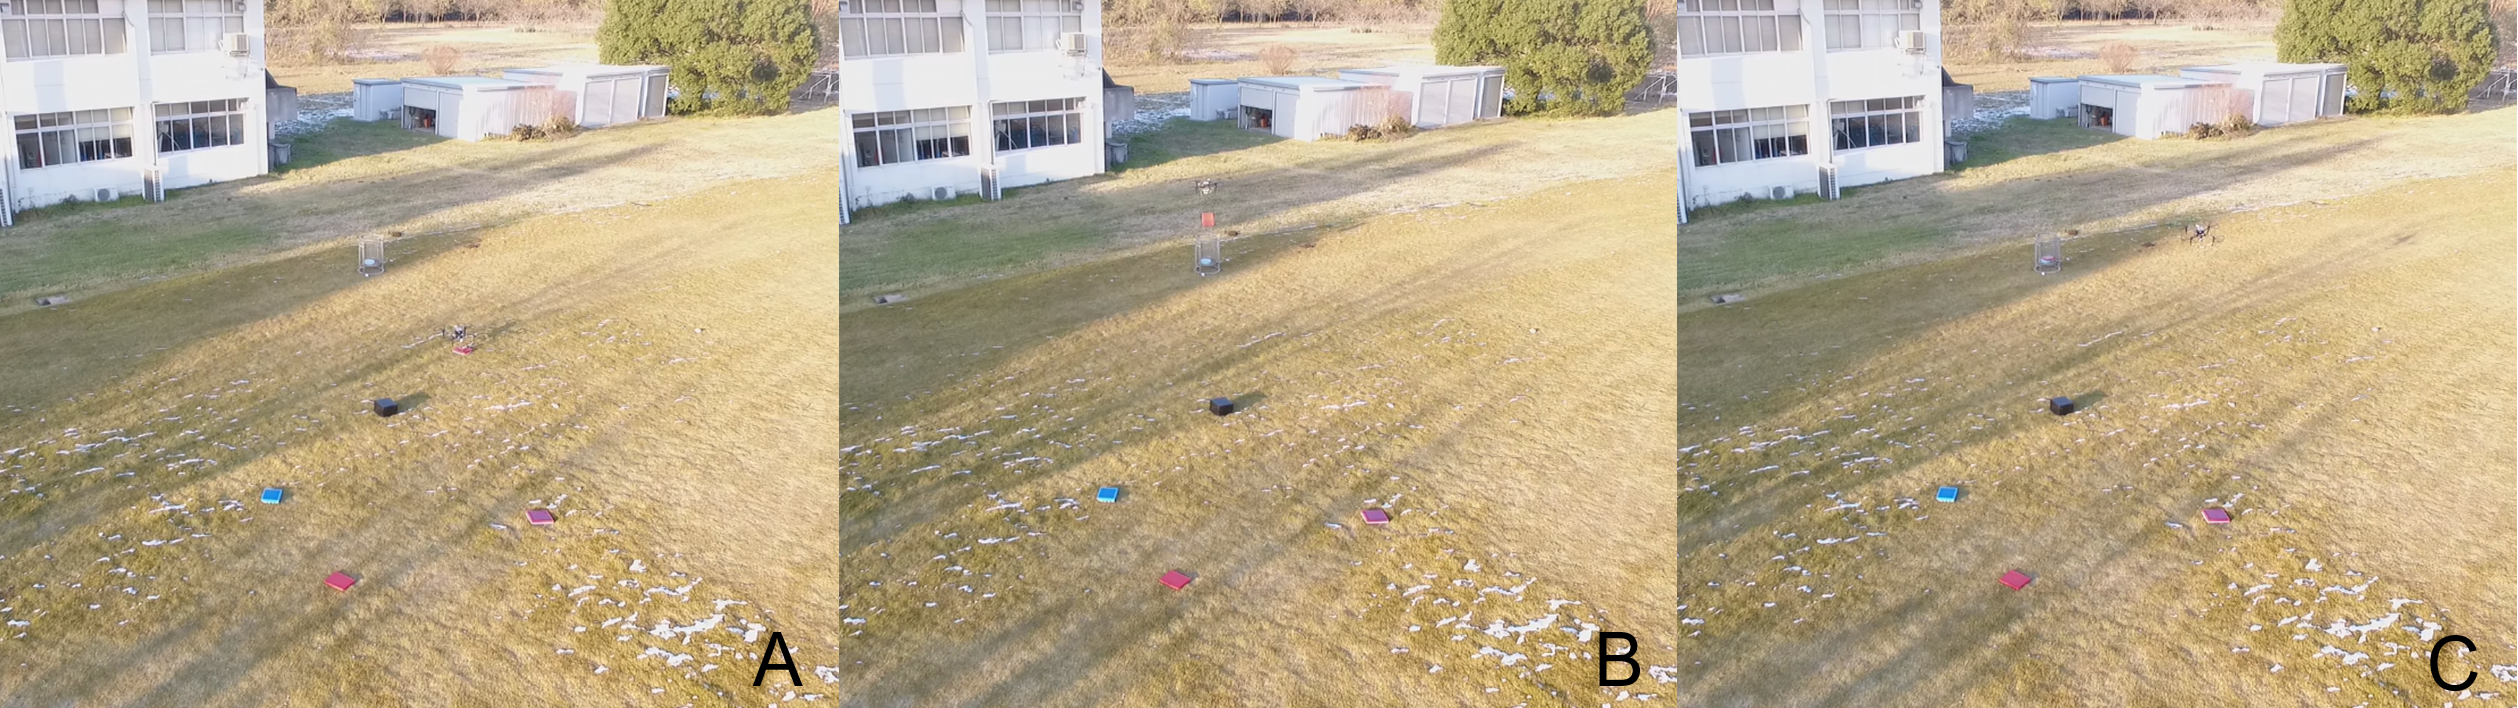
\includegraphics[keepaspectratio=true, width=1\linewidth, height=0.3\textheight]
    {sections//task3//images//teleop.png}
      \end{center}
    \caption{Pick, Place and Search in Teleoperation(A: Pick an object, B: Place the object back to a tray box, C: Search and approach to an object)}
    \label{task3tele}
    \end{figure*}

Four touch sensors are equipped on the gripper with the electromagnets to detect the contacts between the object and the gripper. Besides, these touch sensors will bring the position information of the gripper compared to the object since sometimes only $2$ or $3$ touch sensors are triggered and then we know the offset of the gripper and the object. 
    
The design of the electromagnet circuits driver is simple since it can be simply regarded as a series connection of a inductor and a small resistor, Darlington Transistor will be enough to driver a electromagnet since the current request is only $200 ma$. Because of the inductor effect, a protection diode is very necessary in the circuits. We designed the circuits board with a $32$ bits micro controller, a Darlington driver IC and both serial, CAN communication interface in the gripper board. We write a ROS node in the board and it can directly report the status of the magnets and touch sensors in the gripper and also receive the orders from the embedded computers. 

\subsection{Teleoperation for Task 3}
At this moment, we only perform the real platform experiment through teleoperation by human beings. When we control the UAV manually to pick the object, we figure out it is not a easy job for real UAV platform compared to the simulation since it is very difficult to control the UAV accurately to approach the object, in addition, the ground effect will unstable the UAV when the UAV is getting close to the ground. We address this problem by hanging the magnet gripper with a spring so that the UAV can pick the object without getting too close to the ground. However this may introduce another problem that the gripper will be shaking whenever the UAV change the velocity, we are also addressing this problem now and try to get a stronger hanging method to make the gripper relatively stable.

We tested on only one UAV and it seems we can pick $5$ static objects within $8$ minutes, the time could be improved if we adopt the semi-autonomous teleoperation method like store the global position of the box to drop the objects and after pick the object, the UAV can directly move to the global position of the aim box.

\subsection{Future Work}
In the next step of task 3 we are going to improve our vision detection method that has been already showed in the gazebo simulation and then put it into the real UAV tasks to make task 3 full autonomous. Also we will design a multi UAVs cooperation strategy for task 3 both for teleoperation and full autonomous.

\end{document}
